\subsection{Studies of data from {\MEarth}}
\protect\label{section:mearth}

A data file of observations from {\MEarth} for {\ross} was obtained, showing
observations taken between 15 April 2015 and 16 November 2015. This are
displayed in Fig. \ref{fig:mearthobs}. A periodogram was obtained over the whole
of the data, as displayed in Fig. \ref{fig:mearthallpgram}.

\begin{figure}[!htbp]
\begin{center}
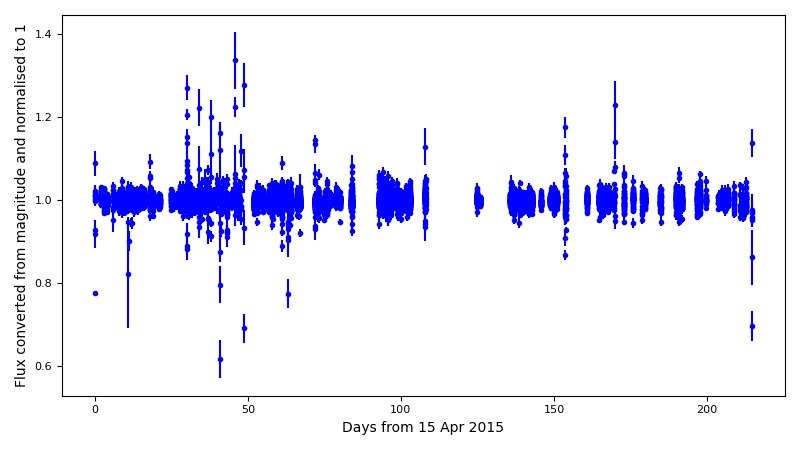
\includegraphics[scale=0.40]{mearth/images/mearthlcurve.png} \\
\vspace{-.5cm}
\end{center}   
\caption{This shows the available observations from
{\MEarth} showing the flux, converted from the reported magnitudes and
normalised to 1, between 15 April and 16 November 2015.}\protect\label{fig:mearthobs}
\end{figure}

\begin{figure}[!htbp]
\begin{center}
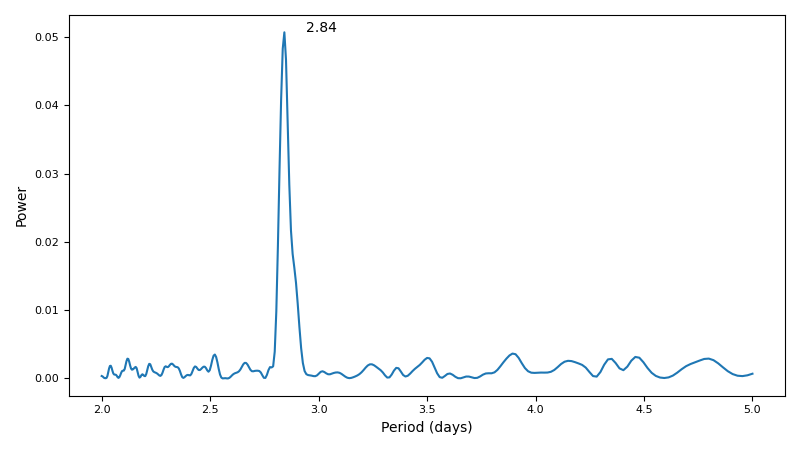
\includegraphics[scale=0.40]{mearth/images/mearthallpgram.png} \\
\vspace{-.5cm}
\end{center}   
\caption{This is a periodogram obtained from
the data in Fig. \ref{fig:mearthobs} for \MEarth. Pruning
of the data of outliers, such as points
exceeding those deviating by more than 2
standard deviations in the data, had
negligible effect on the results.}\protect\label{fig:mearthallpgram}
\end{figure}

The period result of 2.85 days is close to that of 2.843 days obtained from
{\MEarth} by \citet{newton18}. However, the analysis of the {\ktwo} data above
would suggest the the period of approximately 7 months is much too large for an
accurate periodogram; the surface features will have evolved during that period.
There is a problem however in that the number of observations per day is
considerably less than for \ktwo, on some days only of the order of 10
observations were made, less if any are excluded as outliers. In Fig.
\ref{fig:mearthwinsizes} is shown the result of the exercise of trying various
window sizes on the data. It is to be noted that the window function, shown in
Fig. \ref{fig:mearthwinfunc} shows a peak close to this value and possibly
interferes with it.

\begin{figure}[!htbp]
\begin{center}
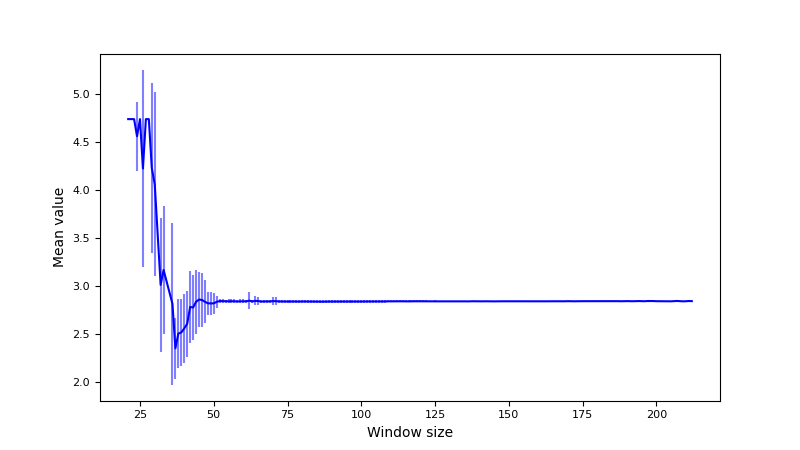
\includegraphics[scale=0.40]{mearth/images/mearthwinsizes.png} \\
\vspace{-.5cm}
\end{center}
\caption{This shows, for the {\MEarth} data for \ross, the development of mean
value of the periodogram main peak (solid line) as the the number of days in
the processing main window is increased. The error bars show the standard
deviations of the mean peak. Points over 2 standard deviations in the data were
omitted from consideration.}\protect\label{fig:mearthwinsizes}
\end{figure}

\begin{figure}[!htbp]
\begin{center}
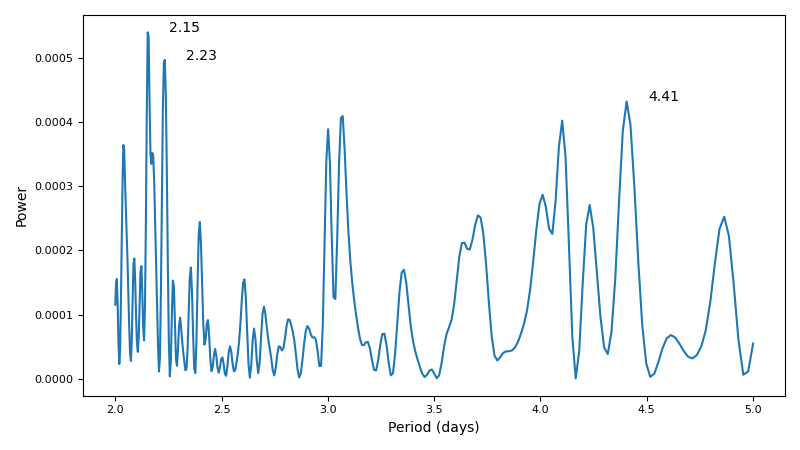
\includegraphics[scale=0.40]{mearth/images/mearthwinf.png} \\
\vspace{-.5cm}
\end{center}
\caption{This shows the window function for
the time series given by the {\MEarth} data
for {\ross} shown in Fig. \ref{fig:mearthobs}
for which the periodogram is shown in Fig.
\ref{fig:mearthallpgram}.}\protect\label{fig:mearthwinfunc}
\end{figure}

